\documentclass[10pt,a4paper]{article}
\usepackage[utf8]{inputenc}
\usepackage[T1]{fontenc}
\usepackage{amsmath}
\usepackage{amsfonts}
\usepackage{amssymb}
\usepackage{graphicx}
\usepackage{listings}
\usepackage{xcolor}
\usepackage{pdfpages}
%\usepackage{blindtext}
\lstset { %
	language=C++,
	backgroundcolor=\color{black!5}, % set backgroundcolor
	basicstyle=\footnotesize,% basic font setting
}

\begin{document}
	\begin{center}
		\begin{LARGE}
			\vspace*{1.5cm}
			\textbf{
				Projektarbeit GPU Matrix-Vektor-Produkt
			}
		\end{LARGE}
		\\ \vspace{1.5cm}
		\begin{large}
			Daniel Emil Giring
			\vfill
			%\textbf{Ausarbeitung über Stencil code}
			%\vfill
		\end{large}
		\begin{normalsize}
			vorgelegt bei\\ \vspace{1.5cm}
		\end{normalsize}
		\begin{normalsize}
			Dr. Ralf Seidler
			\\ \vspace{1.5cm}
			
			Fakultät für Mathematik und Informatik\\
		\end{normalsize}
		\vfill%space{1.5cm}
		\begin{figure}[h]
			\centering
			%\ludegraphics[scale=0.5]{logo.jpg}
			\centering
		\end{figure}
		\vfill%{1.5cm}
		Friedrich-Schiller-Universität Jena
		\\ \vfill%{1.5cm}
	\end{center}
	
	\newpage
	\tableofcontents
	\newpage
	\section{Motivation}
	Matrix-Vektor-Operationen sind Elementar für eine Vielzahl von Berechnungen. Daher ist es von großer Bedeutung diese zu optimieren um Rechenzeit und andere Ressourcen zu sparen. Bei Matrix-Vektor Operation werden viele, bis auf den Indize, gleiche Operationen durchgeführt. Daher eignen sich Grafikarten gut für diese, da GPU sehr effizient bei hochparallelen Anwendungen mit gleichen Operationen sind. Im folgenden werden vier Algorithmen zu Matrix-Vektor vorgestellt, deren Implementierung in Cuda besprochen und deren Performance diskutiert sowie ein Vergleich zu einer CPU Implementierung gezogen wird.
	\section{Algorithmen zur Matrix-Vektor-Operation}
	Aus der linearen Algebra kennen wir das Matrix-Vektor-Produkts wie folgt: Sei $A \in \mathbb{R}^{n\times n}$, $x\in \mathbb{R}^n,$. Dann errechnet sich das Matrix-Vektor-Produkt wie folgt: $ b=Ax, b_j=\sum_{i=1}^n a_{i,j} \cdot x_i$. In den folgenden Implementierungen des Matrix-Vektor-Produkts auf Grafikkarten bekommt jeder thread ein Produkt $a_{i,j}\cdot x_i$ zur Berechnung. Diese Produkte werden dann mittels einer Summer über $i$ reduziert, sodass das Endergebnis in einen Vektor $b$ gespeichert werden kann.
	\subsection{Sharedmemory mit wiederholten Aufruf des Kernels, Kernel 1}
	Für diese Implementierung benötigen wir neben einer $n\times n$ Matrix $A$ und eine $n$-dimensionalen Vektor $x$ einen Speicher für das Ergebnis und die Zwischenergebnisse buff, eine boolvariable doComputation sowie eine Größe toreduce.\\
	Bevor ein Kernel gestartet werden kann muss eine Blockgröße und ein grid definiert werden.
	Da wir mit einer zweidimensionalen Matrix rechnen eignen sich zweidimensionale Threadblöcke.
	In meiner Implementierung kann der Benutzer die Größe der Threadblöcke selbst einstellen, wobei sx die Anzahl der Spalten und sy die Anzahl der Zeilen eines threadblockes darstellt.
	Aus Performancegründen ist es wichtig für sx und sy zweier Potenzen einzugeben. Außerdem muss beachtet werden, dass $sx\cdot sy\leq 1024$, da ein Threadblock maximal 1024 threads enthalten kann. Die Anzahl an Thread-Blöcken, welche gestartet werden, werden in der dim3 Variable grid bzhw, itgrid gespeichert. Dies wird hier auch wieder in zwei Dimensionen dargestellt, da man somit die zweidimensionale Matrix gut in zweidimensionale Blöcke aufteilen kann. \\ 
	Am Anfang wir die boolvariable doComputation auf true gesetzt, toreduce auf $n$, da jeweils $n$ Produkte zu einer Summe zu reduzieren sind. Dem Kernel wird die Matrix $A$, $x$, doComputation, die Anzahl der Spalten der Matrix (size), sowie toreduce übergeben. Nun kann der Kernel das erste mal gestartet werden.\\
	Es werden bei der ersten Ausführung des Kernels size/sx*size/sy viele Threadblöck gestartet. Mann kann sich die Gesamtheit der Threadblöcke wieder wie eine Matrix vorstellen. In jedem Threadblock wird zunächst von den verschiedenen threads das Produkt $a_{i,j}*x_i$ ausgerechnet. Dabei wird die Matrix $A$ so aufgeteilt, dass die verschiedenen Threadblöcke wie ein Gitter über der Matrix liegen. Somit wird jeder Matrixeintrag $a_{i,j}$ in genau einen Threadblock von genauen einen Thread mit dem dazugehörigen Vektoreintrag $x_i$ multipliziert wird. Sei $A$ eine $n*n$ Matrix, so starten wir $n/sx*n/sy$ Threadblöcke der Größe $sx*sy$. Jeder Threadblock rechnet somit $sy$ Zeilen der Länge $sx$ aus A. 
	 Das Ergebnis dieser Multiplikation schreiben die Threads dann in einen shared Memory innerhalb des Threadblocks. Der shared Memory wird so indiziert, dass dieser wieder als Matrix der Größe $sx$*$sy$ gelesen werden kann. Dabei werden Produkte in eine Zeile geschrieben, beide den die Faktoren $a_{i,j}$ auch in der Ursprungsmatrix $A$ innerhalb einer Zeile standen. Über diese Zeile kann jetzt innerhalb des threadblocks reduziert werden. Dafür wird sich die Reduzierung mittels Pointerarithmetik zu Nutzen gemacht. Jede Zeile wird in zwei Hälften geteilt, jeder Zeileneintrag ist einem Thread zugeordnet. Sei $z$ gleich die länge der Zeile, jeder Thread mit threadId.x $i$, $i<z/2$ addiert auf den Wert in Spalte $i$ den Wert aus Spalte $i+z/2$ auf. Ist dies getan wird die vorderen Hälfte der Spalte wieder in zwei Hälften geteilt und das selbe Verfahren auf die vordere Zeile angewendet. Dies wird solange durchgeführt, bis am Ende eine Zeile der länge 1 übrig bleibt. Diese liefert dann den Reduzierten Wert der Zeile. 
	 \\ Damit liefert jeder threadblock als Zwischenergebnis ein Spaltenvektor der Größe Länge $sy$. Diese Spaltenvektoren werden jetzt in einem Zwischenspeicher buff geschrieben. Dabei werden die Ergebnisse der untereinanderliegenden Threadblöcke in gleicher Reihenfolge in buff untereinander, die Ergebnisse der nebeneinanderliegenden Threadblöcke in buff nebeneinander gespeichert. Das Zwischenergebnis ist eine Matrix mit $size/sx$ vielen Spalten und $size$	vielen Zeilen. \\
	 Diese Matrix können wir nun wieder an den Kernel übergeben, dafür müssen wir zunächst noch ein paar Vorbereitungen treffen. Da wir von allen Einträgen $a_{i,j}$ das Produkt mit der entsprechenden Vektorkomponente ausgerechnet haben, wird die Variable doComputation auf false gesetzt. Da im Zwischenergebnis nur noch $size/sx$ viele Zeileneinträge zu reduzieren sind, wird toreduce auf size/sx gesetzt. Da das Zwischenergebnis nur toreduce=$size/sx$ viele Spalten besitzt werden nun weniger Threadblöcke in Zeilen benötigt. Somit wird die x. dimension des grids auf toreduce/sx gesetzt.(toreduce viele Einträge sind pro Zeile zu reduzieren, sx viele Zeileneinträge pro threadblock). buff, welcher das Zwischenergebnis enthällt, toreduce, doComputation und size wird an den kernel übergeben. Da doComputation auf false gesetzt ist werden im Kernel die zu den threadblock gehörigen Matrixeinträge des Zwischenspeichers buff direkt in den shared Memory geschrieben und es muss keine Berechnung dafür durchgeführt werden. Nun wird wie im ersten Schritt über die Zeilen des Shared Memory reduziert. Das Zwischenergebnis eines Threadsblocks ist wieder ein Spaltenvektor mit $sy$ vielen Spalten. Die Spaltenvektoren werden wieder in den Zwischenspeicher buff geschrieben, wobei wir die Spaltenvektoren der Threadblöcke untereinander untereinander gespeichert werden, die Spaltenvektoren der Threadblöcke nebeneinander werden wieder nebeneinander gespeichert. 
	 Das Zwischenergebnis hiervon stellt ein Matrix mit $sy$ vielen Zeilen und $toreduce/sx$ vielen Spalten dar.
	 Am Ende wird toreduce dividiert durch $sx$ da im neuen Zwischenergebnis nur noch $toreduce/sx$ viele Zeileneinträge reduziert werden müssen. Dieses Verfahren wenden wird solange an bis $toreduce=1$. Ist dies erreicht, so haben wir alle Zeileneinträge auf eine Spalte reduziert, sodass wir das die vorderste Spalte des Zwischenergebnis in das Endergebnis speichert können.
	 \subsection{Sharedmemory mit Atomics, Kernel 2}
	 In der zweiten Methode wird der Kernel nur einmal aufgerufen. Ähnlich wie in der Methode, in der wir nur mit shared Memory gearbeitet haben, wird hier zunächst die Matrix auf threadblöcke aufgeteilt, die entsprechenden Multiplikation werden in den Threadblöcken ausgeführt und jede threadblock hat als Zwischenergebnis einen Spaltenvektor der Größe $sy$. Jeodch werden die Einträge der Spaltenvektoren, der verschiedenen threadsblocks, welche aus der selben Zeile der Ursprungsmatrix hervorgehen, auf einen Wert in einem Speicher buff mittels atomicAdd Operationen aufaddiert. Somit liefert nach diesem Kernel buff einen Spaltenvektor der Länge $sy$, welche das Matrix-Vektor-Produkt enthält.
	 \subsection{Nur Atomic Operationen, Kernel 3}
	 Ähnlich wie in den anderen Methoden bekommt hier wieder jedem Eintrag aus der Matrix $A$ genau ein thread zugeordnet, der das Produkt mit der entsprechenden Vektor Komponente ermittelt. Der speichert das Produkt in eine lokale Variable addsc ab. Es wurde vorher ein Speicher buff angelegt, welcher so viele belegbare Speicheradresse besitzt, wie die Matrix $A$ Zeilen. Threads, welche das Produkt mittel des Matrixeintrag aus der gleichen Spalten errechnet haben addieren ihr Ergebnis jetzt auf den entsprechenden Eintrag in der variablen buff auf, sodass buff am Ende ein Spaltenvektor, welcher dem Matrix-Vektor Produkt entspricht, liefert.
	 \subsection{Intra grid Groups, Kernel 4}  
	 In der Methode mit Intra grid Groups sollen sich Threadblöcke untereinander synchronisieren. Damit dies funktioniert kann der Kernel nur eine gewissen Größe an Threadblöcken Gleichzeit starten. Um die maximale Anzahl an threadblöcken, welche sich synchronisieren können herauszufinden gibt es in cuda den Befehl:
	 \begin{lstlisting}
	 	cudaOccupancyMaxActiveBlocksPerMultiprocessor(&numBlocksPerSm,kernel,sx,0);
	 \end{lstlisting}
 	welcher die Anzahl an maximalen verwendbaren Threadblöcken in die Integer variable numBlocksPerSm schreibt. Ich habe mich in der Implementierung dafür entschieden, dass die verschieden Threadblöcke über die Zeilen gehen, wohin hingegen entlang der Spalten nur ein Threadblock untereinander stehen wird. Folglich wurde das grid wie folgt definiert:
 	\begin{lstlisting}
 		grid.y=1;
 		grid.x=(int)ceilf(numBlocksPerSm);
 	\end{lstlisting}
 	Die Blockgröße hingegen kann wieder vom Benutzer eingelesen werden.\\
 	Neben den Anderen Größen muss natürlich nun auch die Größe numBlocksPerSm an den Kernel übergeben werden. \\
 	Innerhalb des Kernel soll wieder jeder thread ein Produkt, bestehend aus einer Matrix und einer Vektorkomponente ausrechnen. Da jetzt aber die Threadblöcke nicht zwangsläufig ausreichen um die gesamte Matrix darzustellen müssen die threads mehrere Produkt ausrechnen. NumberBlocks entspricht der Größe numBlocksPerSm welche an dem Kernel übergeben wurde. Da Numberblocks viele Threadblöcke über das Grid in x.Dimension gestartet werden, und blockdim.x viele threads mit der gleichen y-Komponente innerhalb eines Threadblocks existieren, könnten somit alle threads nur blockDim.x$\cdot$ numberBlocks viele Produkte erstellen, wenn jeder Thread nur ein Produkt ausrechnen würde. Daher wird die Anzahl an Produkte, die jeder thread bei konstanter $y$ Komponente errechnen muss in $lx$ gespeichert.
 	\begin{lstlisting}
 		 int lx=size/(numberBlocks*blockDim.x);
 		if(size % numberBlocks*blockDim.x != 0)
 		lx++;    
 	\end{lstlisting}
 	Ähnlich verhält es sich mit den Produkten die jeder Thread in mit gleichbleibender $x$ Komponente in $y$ Richtung errechnen muss.
 	\begin{lstlisting}
 		int ly=size/(blockDim.y);
 		if(size % blockDim.y != 0);
 		ly++;        
 	\end{lstlisting}
 	Somit kann nun mit den Threadblöcken über die Matrix iteriert werden.
 	\begin{lstlisting}
 	for(int h=0;h<ly;h++){
 		for(int g=0;g<lx;g++){
 			int i=threadIdx.x+blockIdx.x*blockDim.x+g*blockDim.x*numberBlocks;
 			int j=threadIdx.y+h*blockDim.y;   
 			Mult+Reduktion im Threadblock
 			
 			 if (threadIdx.x==0){
 				atomicAdd(&buff[j],sm[threadIdx.y*blockDim.x]);
 				//buff[j]+=sm[threadIdx.y*blockDim.x];
 			} grid.sync();
 		}
 	}
 	\end{lstlisting}
 	Innerhalb der zweiten forschleife wird innerhalb eines Blockes genauso für die Errechnung der Produkte und der Reduktion vorgegangen wie in Kernel1 bzw. Kernel 2.\\
 	Die ursprünglicher Idee war über eine einfache Addition die verschiedenen Threadblöcke in die Variable buff schreiben zu lassen und danach die Threadblöcke zu synchronisieren. Dies hat leider nicht funktioniert sodass ich die Reduktion über die Threadblöcke wieder mit atomicAdd ausgeführt habe. Dies hat zur Folge, dass diese Implementierung nur ein Spezialfall von Kernel2 ist.
	 \subsection{Shuffle}
	 Eine weitere Methode zur Lösung des Problems ist die Verwendung von shuffle Operationen. Diese Bedarf aber einiges mehr an Implementierungsaufwand und wird daher in dieser Stelle nicht näher erläutert. Jedoch ist diese Methode deutliche performanter auf Grafikkarten als die bisher gezeigt sodass ich sie nicht unerwähnt lassen möchte.

	 \section{Performance}
	 \subsection{Verwendete Grafikkarten}
	 Für die Performancemessungen der Algorithmen wurden die Grafikkarten des Lehrstuhls Nvidia GTX780, Nvidia RTX2070super und der das Ara-Clusters Nvidia P100 verwendet. Alle Berechnung wurden mit Daten des Datentyp floats, also in Single Precision ausgeführt.\\
	 Die Angaben zur theoretischen Performance in Table \ref{GPU Daten} der GTX780, P100 sind Herrstellerangaben. Die theoretische Performance der RTX2070super errechnet sich durch: $$\text{SP Performance}= \text{fma}\cdot \# \{\text{Cuda Cores}\} \text{Takt}\\
	 =2\cdot 2560*1,61 Ghz\\
	 =8243 GFlops$$
	 \begin{table}
	 	\centering
	 	\begin{tabular}{llll}
	 		\textbf{Model}  & \textbf{cuda Cores} & \textbf{Takt GHz}  & \textbf{theo. SP. Performace} \\
	 		GTX780           & 2304       & 0,87 (9 Boost) & 3976 GFlops   \\
	 		P100       & 3584 & 1,33 (1,48 Boost) &9400     GFlops        \\
	 		RTX2070super        & 2560 & 1,61 (1,77 Boost) &   8243 GFlops         \\
	 	\end{tabular}
	 	
	 	\caption{GPU Daten}
	 	\label{GPU Daten}
	 	% Verweis im Text mittels \ref{tbl:beispieltabelle}
	 	
	 \end{table}
 	\subsection{Problemgröße}
 	Die Matrixvektormultiplikation wurde in den Performancemessungen auf einer Matrix der Größe $\text{size}\cdot \text{size}$ mit einem Vektor der Dimension size durchgeführt. Dabei galt $size=1024 \cdot n, n\in\{1,2,4,8,16\}$
	 \subsection{Vergleich der Algorithmen}
	 \subsection{Kernel 3}
	 Auf alle Grafikkarten ist Kernel 3, welcher nur Atomic Operationen zur Reduktion benutzt, der Langsamste. Bei Verwendung der Atomic Operation müssen verschiedene threads auf die selben Speicherzellen schreiben, welche keinen geteilten Speicher enthalten. Dies hat zur Folge, dass die entsprechenden Speicherzellen immer wieder neu von threads geladen und beschrieben werden müssen während des die Anderen threads warten müssen, bis sie auf den Speicher zugreifen können. Dieses Problem tritt bei Kernel 3 bei jeder Addition auf, sodass für die Addition weder die threads innerhalb eines threads Blocks, noch die threads über die Threadblöcke verteilt, welche auf die selbe Matrix Zeile zugreifen, parallel addieren können. Das Resultat ist eine recht langsame Performance von maximal 13 GFlops auf der RTX2070super (Abb. \ref{Ausführung Kernel3, RTX2070super }), 4GFlops auf der P100 (Abb. \ref{Ausführung Kernel3, P100 }) und 2,2 GFlops auf der GTX780.(Abb. \ref{Ausführung Kernel3, GTX780 })\\
	 \subsection{Intragrids}
	 Die Methode mit intragrids zeigt eine etwas, aber noch nicht viel schnellere Methode als die des Kernel 3. So erreicht die RTX2070super bis zu 19Gflops, die P100 bis zu 11 GFlops. Auf der GTX780 ist die eine korrekt Ausführung des Kernels 4 leider noch nicht möglich.\\
	  \subsection{Kernel 1 und 2}
	 Deutlich schneller hingegegen sind die Ausführungen von Kernel 1 und 2.
	 Interessant zu beobachten ist, dass auf der GTX780 Kernel 1 und Kernel 2 ähnlich schnell sind. Auf der RTX2070super ist Kernel 2 meist etwas schneller als Kernel 1. Auf der P100 hingegen ist Kernel 1 hingegen deutlich schneller als Kernel 2. Ein mögliche Erklärung hierbei findet sich anhand der Hardwarespezifikationen. Die P100 hat deutlich mehr Cuda Cores als die GTX780, RTX2070super, wodurch sie mehr Threadblöcke gleichzeitig starten kann. Das hilft ihr bei der Ausführung von viele Threadblöcke, also auch beim Wiederaufruf des Kernels. Die RTX2070super ist zudem höher getaktet als die P100, was ihr bei den Atomic Operationen zu Gute kommt. Jedoch lässt es sich nicht allein auf dieses Argument herunterbrechen, da die GTX780 einen deutlich niedriger Taktet als die anderen beiden GPUs besitzt.\\
	 Somit liefert die P100 mit dem Kernel 1 bis zu 70 Gflops,(Abb. \ref{Ausführung Kernel1, P100 }) mit dem Kernel 2 bis zu 48 GFlops. (Abb.\ref{Ausführung Kernel2, P100 })\\
	 Die RTX2070super liefert mit dem Kernel 1 bis zu 33 Gflops,(Abb.\ref{Ausführung Kernel1, RTX2070super }) mit dem Kernel 2 bis zu 47GFlops.\ref{Ausführung Kernel2, RTX2070super }
	 Auf der GTX780 erreicht man mit dem Kernel 1 bis zu 21 Gflops,(Abb.\ref{Ausführung Kernel1, GTX780 }) mit der Kernel 2 bis zu 19  Gflops. (Abb.\ref{Ausführung Kernel2, GTX780 })
%	 \begin{figure}[ht]
%	 	\centering
	 
%%	\label{GPU Vergleich Kernel 1}
%	\end{figure}
	 \subsection{Shuffle}

	%\blindtext
	\begin{figure}
		\includegraphics[page=8,scale=0.8]{../Diagramme/allshared_changei.pdf}
		
		\caption{Ausführung Kernel 1, P100 }
		\label{Ausführung Kernel1, P100 }
	\end{figure}
	
	\begin{figure}
		\includegraphics[page=2,scale=0.8]{../Diagramme/allshared_changei.pdf}
		
		\caption{Ausführung Kernel 1, RTX2070super }
		\label{Ausführung Kernel1, RTX2070super }
	\end{figure}
	
	\begin{figure}
		\includegraphics[page=5,scale=0.8]{../Diagramme/allshared_changei.pdf}
		
		\caption{Ausführung Kernel 1, GTX780 }
		\label{Ausführung Kernel1, GTX780 }
	\end{figure}
	
	
	\begin{figure}
	\includegraphics[page=8,scale=0.8]{../Diagramme/sharedatomic_chagei.pdf}
	
	\caption{Ausführung Kernel 2, P100 }
	\label{Ausführung Kernel2, P100 }
	\end{figure}

	\begin{figure}
		\includegraphics[page=2,scale=0.8]{../Diagramme/sharedatomic_chagei.pdf}
		
		\caption{Ausführung Kernel 2, RTX2070super }
		\label{Ausführung Kernel2, RTX2070super }
	\end{figure}

	\begin{figure}
		\includegraphics[page=5,scale=0.8]{../Diagramme/sharedatomic_chagei.pdf}
		
		\caption{Ausführung Kernel 2, GTX780 }
		\label{Ausführung Kernel2, GTX780 }
	\end{figure}
	
	\begin{figure}
		\includegraphics[page=8,scale=0.8]{../Diagramme/onlyatomic_changei.pdf}
		
		\caption{Ausführung Kernel 3, P100 }
		\label{Ausführung Kernel3, P100 }
	\end{figure}
	
	\begin{figure}
		\includegraphics[page=2,scale=0.8]{../Diagramme/onlyatomic_changei.pdf}
		
		\caption{Ausführung Kernel 3, RTX2070super }
		\label{Ausführung Kernel3, RTX2070super }
	\end{figure}
	
	\begin{figure}
		\includegraphics[page=5,scale=0.8]{../Diagramme/onlyatomic_changei.pdf}
		
		\caption{Ausführung Kernel 3, GTX780 }
		\label{Ausführung Kernel3, GTX780 }
	\end{figure}
	
	
	
	%\blindtext
	 Die schnellste Methode findet sich jedoch im Algorithmus mit shuffle Operationen, welcher nochmal eine bis zu vier mal bessere Performance liefert. So erreicht man auf der RTX2070super bis zu 190, auf der P100 sogar bis zu 237 GFlops.
	 \subsection{Vergleich der Grafikkarten}
	  \subsubsection{Kernel1}
	  Bei der Verwendung des Kernel1 ist die P100 deutlich schneller als die RTX2070super und die GTX780. Hierbei wird vor allem die größere Anzahl an Cuda Cores ihr helfen, da somit mehr Threadblöcke gleichzeitig ausgeführt werden können.
	  \subsubsection{Kernel 2}
	  Bei der Ausführung von Kernel 2 liefert die P100 und die RTX2070super eine vergleichbare Performance. 
	  Die GTX780 ist deutlich langsamer als die anderen Karten was auf die geringer Anzahl an Cuda Cores und den geringer Takt zurückzuführen ist.
	  \subsection{Atomic Operationen}
	  Hier ist die RTX2070super deutlich schneller als die anderen beiden GPUs. Der schnellere Takt wird einen großen Einfluss dabei gespielt haben.
	  \subsection{Einfluss der Problemgröße}
	  \subsubsection{Kernel 1 und Kernel 2}
	  Bei den meisten Versuchen bei der Verwendung von Kernel 1 und Kernel 2 ist mit Vergrößerung der Problemgröße die Compute performance leicht gestiegen. Ein signifikanten Anstieg ist aber meist nicht zu sehen. Vereinzelt gab es aber auch hier leicht Abfälle der Performance mit größerer Problemgröße
	  \subsubsection{Kernel 3}
	  Besonders bei der P100 fällt die Performance mit Vergrößerung der Problemgröße bei Verwendung von Kernel 3 ab.(Abb. \ref{Ausführung Kernel3, P100 })\\ Bei der GTX780 ist ein leichter Verfall der Performance mit Vergrößerung der Problemgröße zu beobachten.(Abb. \ref{Ausführung Kernel3, GTX780 })\\
	  Bei Verwendung der RTX2070super je nach Threadblockgröße (sx) ein leichter oder starker Abstieg der Performance mit Vergrößerung der Problemgröße zu beobachten. (Abb. \ref{Ausführung Kernel3, RTX2070super })
	  \subsection{Einfluss der Blockgröße}
	  Die Performance Messung wurden mit fester Blockgröße bezüglich der Zeilen eines Threadsblocks $sy=16$ aber Variabler Blockgröße $sx$ bezüglich der Spalten eines Threadsblocks durchgeführt. Dabei war $sx\in\{4,8,16,32,64\}$. Je nach Kernel, GPU und Problemgröße war zwischen den verschieden Blockgröße $sx$ ein Performanceunterschied vom Faktor bis zu vier zu sehen. (z.B. GTX780, kernel 1 Abb. \ref{Ausführung Kernel1, GTX780 }) Interessant dabei zu beobachten war, dass bei Kernel 1 und 2 auf der RTX2070super die Ausführung mit $sx=8$, auf der GTX780 meist die Ausführung mit $sx=16$ am schnellst war. Auf der P100 hingegen war für Kernel 1 bei kleiner Problemgröße die Ausführung für $sx=8$ am schnellsten und für große Problemgröße die Ausführung mit $sx=16$ leicht schneller als die mit $sx=8$. Bei Kernel 2 hingegen war die Ausführung mit $sx=32$ deutlich schneller auf der P100 als die anderen Ausführungen.(Abb. \ref{Ausführung Kernel2, P100 }) Ein Grund hierfür ist, dass die P100 recht langsam bezüglich der Atomic add Operationen ist. Wird $sx$ größer, so müssen weniger Atomic Add Operationen durchgeführt werden, da die Threadblöcke größer werden, wodurch man weniger threadblöcke benötigt und nur zwischen den Threadblöcken die Atomicadd Operation ausgeführt wird. Eine weiter Erhöhung der Blockgröße auf $sx=64$ führt jedoch zu einer schlechteren Performance. \\
	  Eine Richtlinie, welche Blockgröße generell Ideal ist konnte ich aber wegen der sehr verschiedenen Ergebnissen auf den verschiedenen Grafikkarten nicht erstellen.
	 
	  \subsection{Einfluss der Größe von Shared Memory/ L1 Memory}
	  Kernel 1, 2 und 3 und wurden mit verschiedenen Cache Konfiguration durchgeführt.
	  \begin{lstlisting}
	  (1)cudaFuncSetCacheConfig(kernel,cudaFuncCachePreferL1);
	  (2)cudaFuncSetCacheConfig(kernel,cudaFuncCachePreferShared);
	  (3)cudaFuncSetCacheConfig(kernel,cudaFuncCachePreferNone);  
	  \end{lstlisting}
		Dabei wird 64 kByte in Shared Memory und L1 Memory aufgeteilt. In Konfiguration 1 wird 48Kbyte dem L1 Speicher, 16 KByte dem shared memory, in Konfiguration 2 wird 16 kByte dem L1 Speicher, 48kByte dem shared memory und in Konfiguration 3 je 32 kByte den beiden Speicher zugeordnet. 
		\\ Zwischen den Ausführungen mit verschieden Shared Memory Konfiguration sieht man meist keine großen Unterschiede. Das liegt daran, dass in jeder Implementierung nur ein shared Memory Objekt im Kernel definiert wurde. Dies hat maximal die Größe $1024\cdot \text {sizeof(float)}$, also ist Maximal 4 kByte groß, sodass er problemlos auch in Konfiguration 1 mit dem kleinen shared Memory klein genug ist um im Speicher zu bleiben.
	  \subsection{Differenz zur theoretischen Peak Performance}
	  Bei allen Algorithmen und allen GPUs ist die erreichte Performance weit von der theoretischen Peak Performance entfernt. So erreicht man mit der P100 im shuffle Algorithmus maximal 237 GFlops, mit Kernel 1 maximal 70 Gflops. Die Performance von Kernel 1 entspricht somit nur ein hundertstel der theoretischen Peakperformance von 9400 Gflops der P100. Die Differenz bei der RTX2070super und der GTX780 liegt in einer ähnlichen Größenordnung. Ein Grund hierfür ist, dass die geladenen Matrixeinträge der Ursprungsmatrix $A$ nur einmal zur Berechnung benutzt werden und auch bei Grafikkarten die Recheneinheiten deutlich mehr Daten verarbeiten könnten, als die Speichereinheiten Daten liefern können. Bei einer Matrix-Matrix-Multiplikation müssen die Daten der Ursprungsmatrix deutlich häufiger verwendet werden als bei einer Matrix-Vektor-Multiplikation, da für $C+=AB$ jede Zeile von Matrix $A$ mit jeder Spalte aus Matrix B multipliziert wird. Somit bin ich in Hausaufgabe 3, der Matrix-Matrix-Multiplikation, auf eine Performance von knapp 600 GFlops mit der RTX2070super gekommen. Dies entspricht der dreifachen Performance der Implemtierung des shuffle Algorithmus (190 GFlops), und sogar der 12-fachen Performance der Implemtierung von Kernel 2(47 GFlops) und der 18 fachen Performance der Implemtierung von Kernel 1 (33 Gflops).
	  \subsection{Performance Vergleich CPU}
	  Eine Single Core CPU Implementation das Matrix-Vektor-Produktes, bei der die Matrix in Teilmatrizen aufgeteilt war für effektiver Transfer bezüglich Cache Lines, hat auf meinem System, mit AMD Ryzen 5 3600, eine Performance zwischen 0,1 und 3 Gflops erreicht. Besonders bei großer Problemgröße war die Ausführung sehr langsam. So hat sie für das Matrix-Vektorprodukt mit Dimension 16*1024 Werte zwischen 0,01 und 0,42 GFLOPS, je nach Größe der Teilmatrix.\\ 
	  Vor der Krise bezüglich der Verfügbarkeit von Grafikkarten hat man für ungefähr den gleichen Preis ein Nvidia RTX2070 super oder einen AMD Ryzen 9 3900X bekommen. Letzterer ist eine 12-core CPU mit einer vergleichbaren single core Performance zum AMD Ryzen 5 3600. \\
	  Geht man von einer Perfekten Parallelisierung das Programms aus und dem Idealfall der Singlecore Impletmentierung von 0,42 GFlops, so erhält man mit dem Ryzen 9 3900X eine Performance von $0,42GFlops*12=5,04 GFlops$. Dies wäre um ein Faktor 9 schlechter, als die Performance des Matrix Vektor Produkts Kernel 2 auf der RTX2070super mit sx=8,size=16*1024, und sogar um ein Faktor 35 schlechter als der shuffle Algorithmus auf der RTX2070super (185 Gflops) für size=16*1024.\\
	  Ähnliches beobachtet man bei der theoretischen Peak Performance. Der AMD Ryzen 9 3900x  unterstüzt AVX2 und FMA Operation. Kann also 2 Operatioen auf 256bit pro Takt ausführen. 256bit entsprechen der Größe von 8 floating Point Datentypen. Die Theoretische performance errechnet sich hierdurch durch:
	  $$\text{SP Performance}=\text{fma}\cdot \#\{\text{Cores}\}\cdot\text{Values per cycle}\cdot \text{Takt}$$ $$=2*12*8*3,8GHz=729,6 GFlops$$
	  Die theoretische Peakperformance des Ryzen 9 3900x liegt ist mit 730GFlops ist um einen Faktor 11 schlechter als die der Nvidia RTX2070super mit theoretischen 8243 GFlops, Table \ref{GPU Daten}. Somit ist auszugehen, dass der Performanceunterschied auch bei weiteren Optimierung des Codes erhalten bleibt. \\ 
	   Anhand dieses Beispiels kann man gut sehen, warum für Berechnungen von großen Matrix-Matrix oder Matrix-Vektorprodukten oft GPUs anstatt CPUs verwendet werden. Bei gleichbleibenden Operationen auf großen Datensätzen bieten die GPUs aufgrund der hohen Anzahl an Cuda-Cores enorme Performance Vorteile gegenüber CPUs. CPUs werden trotzdem weiterhin eine zentrale Rolle in Computer spielen, da sie deutlich schneller bei der Ausführung von vielen verschiedenen Instruktionen nacheinander sind und der Großteil der Software auf CPU Ausführung programmiert ist. GPUs eignen sich aber wunderbar als Erweiterung für große Berechnungen.
	   \section{Fazit}
	   GPUs eignen sich sehr gut für die Berechnung eines Matrix-Vektor Produkts. Mit Implemtierung wie den shuffle Algorithmus erhällt man ein effektiv nutzbare Performance welche nahe an der Theoretischen Peak Performance von CPUs liegt. Die neue Grafikkarten von Nvidia der Ampere liefern nochmals deutlich mehr Cuda Cores, sodass der Vorteil von GPUs gegenüber CPUs bei solchen Berechnungen nochmal gestärkt wird und sie mittelfristig unverzichtbar im HPC sind.  	     
	 \section{Quellen} 
	 - https://www.nvidia.de/gtx-700-graphics-cards/gtx-780/
	 -https://www.computerbase.de/2016-04/nvidia-tesla-p100-gp100-als-grosser-pascal-soll-all-in-fuer-hpc-markt-gehen/
%	 -https://en.wikichip.org/wiki/amd/ryzen_9/3900x
	\newpage
	\begin{thebibliography}{2}
		\addcontentsline{toc}{chapter}{Quellenverzeichnis}
		\bibitem{manuel} \textit{https://www.nvidia.de/gtx-700-graphics-cards/gtx-780/},.
		\bibitem{manuel}\textit{ https://www.computerbase.de/2016-04/nvidia-tesla-p100-gp100-als-grosser-pascal-soll-all-in-fuer-hpc-markt-gehen/} \label{P100 Performance}.
		\bibitem{manuel} \textit{https://en.wikichip.org/wiki/amd/ryzen\_9/3900x}
	\end{thebibliography}
\end{document}